\chapter{Controllo attivo di un processo}


\section{Generalit\`{a} sul concetto di Sistema}

Un sistema \`{e} un complesso in cui si possono definire grandezze che prendono il nome di variabili(nel tempo).

\subsection{Modello matematico}

Il modello matematico descrive un sistema con equazioni e parametri, le due distinzioni principali sono:
\begin{itemize}
  \item MIMO: sistemi multivariabili
  \item SISO: sistemi scalari
\end{itemize}

\subsection{Sistema statico e dinamico}
Un sistema \`{e} statico quando l'uscita al tempo $t$ dipende soltanto dal valore all'ingresso al tempo $t$.

Un sistema \`{e} dinamico quando l'uscita al tempo $t$ dipende dal segnale all'ingresso compreso nel periodo $(-\infty, t)$.


Nel caso di sistemi dinamici vengono introdotti i concetti di:
\begin{itemize}
  \item sistma in quiete
  \item sistema in condizioni asintotiche
  \item sistema a regime
\end{itemize}

\subsection{Insieme dei \textit{behaviors}}

$\beta$ \`{e} l'insieme di tutte le possibili coppie causa effetto associate al sistema.




\subsection{Linearit\`{a}}
Un sistema si dice lineare se rispetta il principio di sovrapposzione degli effetti.

\subsection{Stazionariet\`{a}}

Un sistema si dice stazionario(invariante nel tempo) se il ritardo(differenza di tempo) $T$ che si ha tra segnale $A$ e segnale 
$B$ sia $\forall T \in \mathbb{R}$


\section{Controllo in azione diretta o in retroazione}

Il controllo attivo \`{e} distinguibile in:
\begin{itemize}
  \item azione diretta(\textit{feedforward}) o ad anello aperto o in catena aperta
  \item retroazione(\textit{feedback}) o ad anello chiuso o in catena chiusa
\end{itemize}

\subsection{Controllo ad azione diretta}
L'azione di comando dipende da:
\begin{itemize}
  \item obiettivo perseguito
  \item informazioni dul modello del sistema controllato
  \item disturbi agenti sul sistema
\end{itemize}


\subsection{Controllo in retroazione}

\begin{itemize}
  \item obiettivo perseguito
  \item informazioni sul modello del sistema di controllo
  \item disturbi agenti sul sistema
  \item variabile controllata
\end{itemize}

\subsection{Confronto tra controllo ad azione diretta e in retroazione}

\begin{figure}[h!]
  \begin{center}
    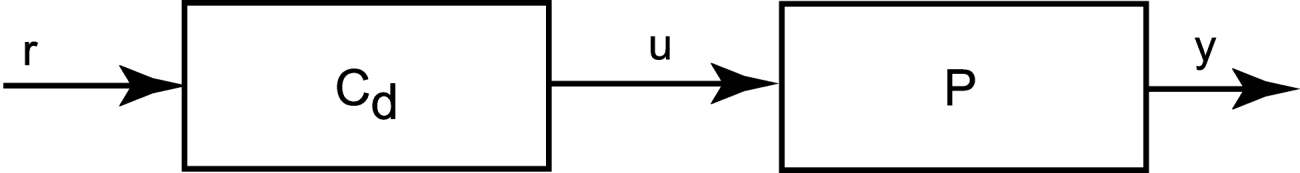
\includegraphics[width=0.5\textwidth]{images/controllo_diretto.png}
  \end{center}
  \caption{Esempio di controllo diretto}
  \label{fig:controllo_diretto}
\end{figure}

Nel caso di controllo diretto come nelal figura qui sopra, la $y$ si ottiene facendo:
\begin{equation}
  y = Pu = P (C_d r) = PC_d r 
  \label{eq:eq_controllo_diretto}
\end{equation}


\begin{figure}[h!]
  \begin{center}
    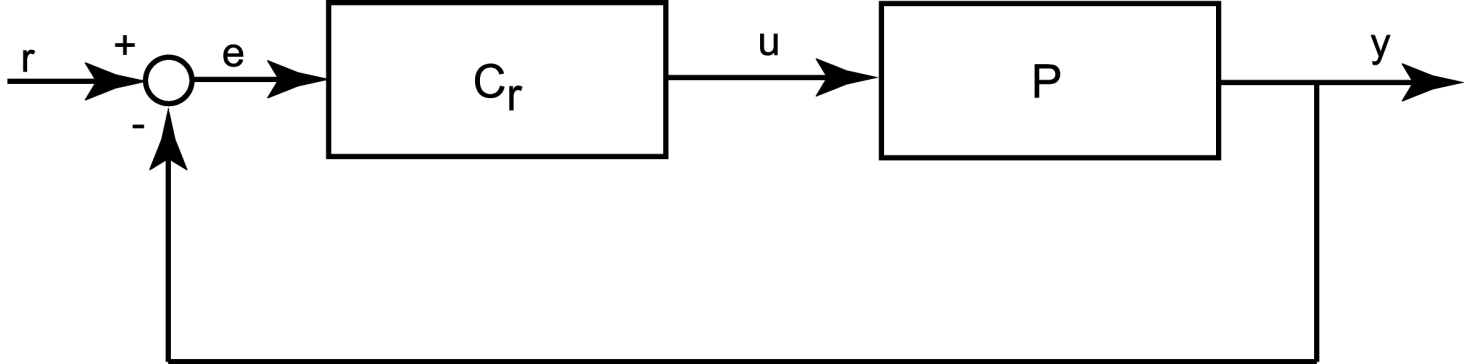
\includegraphics[width=0.5\textwidth]{images/controllo_retrazione.png}
  \end{center}
  \caption{Esempio controllo in retroazione}
  \label{fig:controllo_retrazione}
\end{figure}

Nel caso si un controllo retrazionato la $y$ si ottiene:

\begin{equation}
  y = \displaystyle\frac{PC_r}{1 + PC_r} \cdot r
  \label{eq:eq_controllo_retrazionato}
\end{equation}





\subsection{Esamina delle strategie di controllo in condizioni di perturbazione}

Nel caso di controllo diretto l'errore si aggira intorno al $\pm 20\%$.

Nel caso di sistema retroazionato l'errore di inseguimento si aggira tra in $0.415\%$ e il $0.621\%$.



